\section{Постановка задачи} \label{p31}
\paragraph{}
 Рассмотрим математическую модель трехзвенного манипулятора, состоящую из трех абсолютно жестких звеньев $G_1, G_2, G_3$, представляющих собой однородные стержни. Манипулятор установлен на неподвижном основании, на которое опирается звено $G_1$. Звено $G_1$ таким образом, может совершать только вращения вокруг вертикальной оси. Звенья соединены между собой двумя идеальными цилиндрическими шарнирами $O_1$, и $O_2$ таким образом, что звенья $G_2$ и $G_3$ могут совершать движения только в вертикальной плоскости. Центр масс $C_1$ звена $G_1$ лежит на луче  $O_1 O_2$. Положение центра масс $C_2$ звена $G_2$ не совпадает с положением шарнира $O_2$. На конце звена $G_3$ находится груз, перемещаемый манипулятором.
 
 Введем обозначения: $q_i (i=1, 2, 3)$ --- углы поворотов звеньев манипулятора; $Q_i (i = 1, 2, 3)$ ---  управляющие моменты относительно осей соответствующих звеньев; $l_i$  ---  длина   $i$-го звена;   $m_i$ --- масса  $i$-го звена;    $m_0$ ---  масса перемещаемого груза;  $m_{30} = m_0 + m_3$; $J_{01}$  ---  момент инерции первого звена относительно оси вращения; $r_2$ и $r_3$ --- соответственно расстояния от центров тяжести второго и третьего звеньев с перемещаемым грузом относительно осей соответствующих звеньев; $g$ --- ускорение свободного падения.
 
 \begin{figure}[h]
 	\centering
 	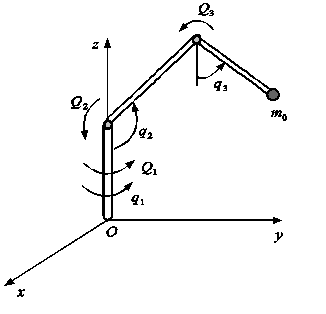
\includegraphics{3chain}
 	\caption{Модель трехзвенного манипулятора}
 	\label{fig:manip1}
 \end{figure}
 
 Кинетическая энергия системы в векторно-матричном виде может быть записана в виде:
 
  \begin{equation*}
  T = \frac12 \dot q^{'} A(q) \dot q, \quad q^{'} = (q_1, q_2, q_3),
  \end{equation*}
  
  \begin{equation*}
  A(q) =
  \begin{pmatrix}
  a_{11} && 0 && 0  \\
  0  && a_{22} && a_{23} \\
  0 && a_{32} &&  a_{33}\\
  \end{pmatrix}
  \end{equation*}
  
  \begin{equation*}
  \begin{array}{l}
  a_{11} = J_{01} + m_2 r_2^2 \sin^2 q_2 + m_{30} (l_2 \sin q_2 + r_3 \sin q_3)^2 \\
  a_{22} = m_2 r_2^2 + m_3 l_2^2 \\
  a_{23} = \frac12 m_{30} l_2 r_3 \cos(q_2 - q_3) \\
  a_{32} = a_{23} \\
  a_{33} = m_{30} r_3^2 \\
  \end{array}
  \end{equation*}
  
  Учитывая действие сил тяжести, уравнения движения можно записать в векторно-матричной форме
    
  \begin{equation}
  A(q) \ddot q + C(q, \dot q) \dot q + K(q) = Q \label{chain3_matrix_form}
  \end{equation}
    
  \begin{equation*}
  C(q, \dot q)= 
  \begin{pmatrix}
  c_{11} && 0 && c_{13} \\
  c_{21} && 0 && c_{23} \\
  c_{31} && c_{32} && 0\\
  \end{pmatrix}
  \end{equation*} 
        
   \begin{equation*}
   \begin{array}{l}
   c_{11} = 2 (m_2 r_2^2 \sin q_2 \cos q_2 + m_{30} (l_2 \sin q_2 + r_3 \sin q_3) l_2 \cos q_2) \dot q_2 \\
   c_{13} = 2 m_{30} (l_2 \sin q_2 + r_3 \sin q_3) r_3 \cos q_3 \dot q_3 \\
   c_{21} = - (m_{30} (l_2 \sin q_2 + r_3 \sin q_3) l_2 + m_2 r_2^2 \sin q_2) \cos q_2 \dot q_1 \\
   c_{23} = \frac12 m_{30} l_2 r_3 \sin(q_2 - q_3) \dot q_3 \\
   c_{31} = - m_{30} (l_2 \sin q_2 + r_3 \sin q_3) r_3 \cos q_3 \dot q_1 \\
   c_{32} = - \frac12 m_{30} l_2 r_3 \sin (q_2 - q_3) \dot q_2 \\
   \end{array}
   \end{equation*}
 
 
   \begin{equation*}
   K^{'} (q) = (0, (m_2 r_2 + m_{30} l_2) g \sin q_2, m_{30} g r_3 \sin q_3)
   \end{equation*}
 
 \markright{\thechapter.\thesection.\hspace{1em}Построение управления}{}
 \label{sec2.3}
 Пусть  $q = (q_1, q_2, q_3)^{'}$ --- вектор обобщенных координат рассматриваемой механической системы и $$X = {q^0(t):[t_0, + \infty) \to R^3, \| q^0(t) \| \le q_0, \| \dot q^0 \| \le g_1,\| q^0(t) \| \le q_0, \| \ddot q^0 \| \le g_2}$$ есть заданное множество программных движений манипулятора в виде ограниченных дважды непрерывно дифференцируемых функций $q = q^0(t)$ с ограниченными производными при $t \in [t_0, + \infty)$.  Символом   $\| \cdot \|$ обозначена евклидова норма вектора.
 Пусть $q^0(t) \in X$ --- какое-либо программное движение системы (\ref{chain3_matrix_form}), реализуемое программным управлением $Q^{(0)}$, так что $Q^{0} (t) = Q(t)$ при $q = q^{0}(t), \dot q = \dot q^{0}(t)$ т.е. имеет место тождество $$A(q^0(t)) \ddot q^0(t) + C(q^0(t), \dot q^0(t)) \dot q^0(t) + K(q^0(t)) \equiv Q^{(0)} (t).$$
 Введем возмущения $x = q - q^0(t)$ и составим уравнения возмущенного движения в векторно-матричном виде:
 \begin{equation}
 A^{(1)}(t, x) \ddot x + C^{(1)}(t, x, \dot x) \dot x + K^{(1)}(t, x) = Q^{(1)}(t, x, \dot x) + Q^{(2)}(t, x, \dot x), \label{chain3_disturb_sys}
 \end{equation} 
 где
 $$
 \begin{array}{c}
A^{(1)}(t, x) = A(x + q^0(t))$, $C^{(1)}(t, x, \dot x) = C(x + q^0(t), \dot x + \dot q^0(t)),\\
K^{(1)} (t, x) = K(q^0(t) + x) - K(q^0(t)),\\
 Q^{(1)}(t, x, \dot x) = Q - Q^{(0)},\\
Q^{(2)}(t, x, \dot x) = (A^{(1)}(t, 0) - A^{(1)}(t, x)) \ddot q^0(t) + (C^{(1)}(t, 0, 0) - C^{(1)}(t, x, \dot x)) \dot q^0(t) 
 \end{array}
 $$
 
 Рассмотрим задачу построения управляющего воздействия $Q^{(1)}(t, x, \dot x)$, при котором невозмущенное движение $\dot x = x = 0$ системы (3.3) было бы равномерно асимптотически устойчиво, или, иначе, управление $Q = Q^{(1)}(t, q-q^{(0)}(t), \dot q - \dot q^{(0)}) + Q^{(0)}$ обеспечивало бы стабилизацию программного движения   системы (\ref{chain3_disturb_sys}).
 
  \section{Приведение манипулятора в заданное программное положение}%
  
  Рассмотрим задачу приведения манипулятора в заданное программное положение $q = q^{0} = const$ без измерения скоростей.
  
  В соответствии с проведенной постановкой задачи получаем
  
  \begin{equation}
  \begin{array}{l}
   q^{0}(t) \equiv q^{0}, \quad (q^{0})^{'} = (q_1^0, q_2^0, q_3^0), \quad \dot q^{0}(t) \equiv U_x, \\
   x_1 = q_1 - q_1^0, \quad x_2 = q_2 - q_2^0, \quad x_3 = q_3 - q_3^0 \label{3chain_dist}
   \end{array}
   \end{equation}
   
   Соответственно, это положение имеет место если
   
    \begin{equation}
     \begin{array}{l}
     Q_1^{(0)} = 0, \\
     Q_2^{(0)} = (m_2 r_2 + m_{30} l_2)g \sin q_2^0 \cos x_2, \\
     Q_3^{(0)} = m_{30} g r_3 \sin q_3^0 \cos x_3 \label{chain3_control_functions}
     \end{array}
    \end{equation}
    
  Возмущенное движение системы описывается уравнением (\ref{chain3_disturb_sys}), в координатах
  
     \begin{equation}
      A^{(1)}(x) = A(q^0 + x), \quad C^1(x, \dot x) = C(q^0 + x, \dot x)
     \end{equation}
     
  Рассматриваемая задача состоит в нахождении управлеющего воздействия
  
     \begin{equation*}
      Q^{(2)} = Q - Q^{(0)}
     \end{equation*}
     
  обеспечивающего глобальную стабилизацию положения (\ref{3chain_dist}) при измерении значений
  
     \begin{equation*}
     x_1 = q_1 - q_1^0, \quad x_2 = q_2 - q_2^0, \quad x_3 = q_3 - q_3^0
     \end{equation*}
     
  Покажем, что поставленная задача решается управляющим воздействием
  
  \begin{equation}
  \begin{array}{l}
  \displaystyle Q_1^{(2)} (x_1) = -k_1 \sin \frac{x_1(t)}{2} - \cos \frac{x_1(t)}{2} \int_{t - h}^{t} p_1^0 e^{s_1^0 (\tau - t)} \left( \sin \frac{x_1(t)}{2} - \sin \frac{x_1(\tau)}{2} \right) d \tau \\
  \displaystyle Q_2^{(2)} (x_2) = -k_2 \sin \frac{x_2(t)}{2} - \cos \frac{x_2(t)}{2} \int_{t - h}^{t} p_2^0 e^{s_2^0 (\tau - t)} \left( \sin \frac{x_2(t)}{2} - \sin \frac{x_2(\tau)}{2} \right) d \tau \\
  \displaystyle Q_3^{(2)} (x_3) = -k_3 \sin \frac{x_3(t)}{2} - \cos \frac{x_3(t)}{2} \int_{t - h}^{t} p_3^0 e^{s_3^0 (\tau - t)} \left( \sin \frac{x_3(t)}{2} - \sin \frac{x_3(\tau)}{2} \right) d \tau \\ \label{chain3_control_int}
  \end{array}
  \end{equation}
  
  где коэффициенты $h > 0, p_j^0 > 0, s_j^0 > 0,$ а $k_j$ удовлетворяет неравенствам
  
  \begin{equation*}
  \begin{array}{l}
  k_1 > 0, \\
  k_2 > - 2 (m_2 r_2 + m_{30} l_2) g \sin q_2^0, \\
  k_3 > - 2 m_{30} g r_3 \sin q_3^0
  \end{array}
  \end{equation*}
  
  Выберем функционал Ляпунова в виде
  
  \begin{equation*}
  \begin{array}{l}
   \displaystyle V(\dot x(t), x_t) = \frac12 (\dot x(t))^{'} A^{(1)} (x(t)) \dot x(t) + \\
   \displaystyle +(m_2 r_2 + m_{30} l_2) g \sin q_2^0 (1 - \cos x_2) + m_{30} g r_3 (1 - \cos x_3) + \\ 
   \displaystyle + 2 k_1 \left(1 - \cos \frac{x_1(t)}{2} \right) + 2 k_2 \left(1 - \cos \frac{x_2(t)}{2} \right) + 2 k_3 \left(1 - \cos \frac{x_3(t)}{2} \right) + \\ 
   \displaystyle + 2 \int_{t - h}^{t} p_1^0 e^{s_1^0 (\tau - t)} \left( \sin \frac{x_1(t)}{2} - \sin \displaystyle \displaystyle \frac{x_1(\tau)}{2} \right)^2 d \tau + \\ 
   \displaystyle + 2\int_{t - h}^{t} p_2^0 e^{s_2^0 (\tau - t)} \left( \sin \frac{x_2(t)}{2} - \sin \frac{x_2(\tau)}{2} \right)^2 d \tau + \\ 
   \displaystyle + 2 \int_{t - h}^{t} p_3^0 e^{s_3^0 (\tau - t)} \left( \sin \frac{x_3(t)}{2} - \sin \frac{x_3(\tau)}{2} \right)^2 d \tau
  \end{array}
  \end{equation*}
  
  Несложно определить, что этот фукнционал удовлетворяет условию 1) теоремы 1.3. Для полной производной этого функционала в силу уравнений (\ref{chain3_disturb_sys}) с учетом (\ref{chain3_control_functions}) - (\ref{chain3_control_int}) находим
  
    \begin{equation*}
    \begin{array}{l}
	\displaystyle \dot V = - 2 \int_{t - h}^{t} p_1^0 s_1^0 e^{s_1^0 (\tau - t)} \left( \sin \frac{x_1(t)}{2} - \sin \frac{x_1(\tau)}{2} \right)^2 d \tau + \\
	\displaystyle + \int_{t - h}^{t} p_2^0 s_2^0 e^{s_2^0 (\tau - t)} \left( \sin \frac{x_2(t)}{2} - \sin \frac{x_2(\tau)}{2} \right)^2 d \tau + \\ 
	\displaystyle + \int_{t - h}^{t} p_3^0 s_3^0 e^{s_3^0 (\tau - t)} \left( \sin \frac{x_3(t)}{2} - \sin \frac{x_3(\tau)}{2} \right)^2 d \tau
    \end{array}
    \end{equation*}
  
  
  Множество $\lbrace \dot V = 0 \rbrace$ состоит из движений $x(\tau) = x(t), t - h \le \tau \le t,$ или $x(t) = const.$ Из уравнений движений находим, что для таких движений должны удовлетворяться соотношения 
  
  \begin{equation*}
	\sin \frac{x_1(t)}{2} \equiv 0, \quad \sin \frac{x_2(t)}{2} \equiv 0, \quad \sin \frac{x_3(t)}{2}
  \end{equation*}
  
  Согласно теореме 1.3 равномерную асимптотическую устойчивость положения $\dot x(t) \equiv 0, x(t) \equiv 0$ или программного положения (3.4).
  
  В соответствии с теоремой 1.2 каждое возмущенное движение системы будет при $t \to + \infty$ неограниченно приближается к положению
  
  \begin{equation*}
  \dot x_k(t) = 0, \quad \sin \frac{x_k(t)}{2} \equiv 0
  \end{equation*}
  
  или
  
  \begin{equation*}
  \dot x_k (t) \equiv 0, \quad x_k(t) = 2 \pi k, \quad k = 1, 3
  \end{equation*} 
  
  Тем самым, можно утверждать о глобальной стабилизации заданного программного движения (\ref{chain3_disturb_sys}).
  
  \section{Стабилизация стационарного вращения манипулятора вокруг вертикальной оси}%
  
  Координата $q_1$, определяющая вращение манипулятора вокруг вертикальной оси является циклической.
  
  Вводим соответствующий циклический импульс
  
  \begin{equation*}
  (J_0 + m_2 r_2^2 \sin^2 q_2 + m_{30} (l_2 \sin q_2 + r_3 \sin q_3)^2) \dot q_1 = v_1
  \end{equation*} 
  
  Вводим функцию Рауса
  
  \begin{equation*}
  \begin{array}{c}
  \displaystyle R = T - \dot q_1 v_1 = \frac12 (m_2 r_2^2 + m_3 l_2^2) \dot q_2^2
  + \frac12 m_{30} l_2 r_3 \cos(q_2 - q_1) \dot q_2 \dot q_3 + \frac12 m_{30} r_3^2 \dot q_3^2 - \\ \displaystyle - \frac12 \frac{v_1^2}{J_0 + m_2 r_2^2 \sin^2 q_2 + m_{30} (l_2 \sin q_2 + r_3 \sin q_3)^2} \equiv R_2 - R_0
  \end{array}
  \end{equation*}
  
  Уравнение движения системы в форме Рауса записано в виде
  
  \begin{equation*}
  \begin{array}{l}
  \displaystyle (m_2 r_2^2 + m_3 l_3^2) \ddot q_2 + \frac12 m_{30} l_2 r_3 \cos(q_2 - q_1) \ddot q_3 + \frac12 m_{30} l_2 r_3 \sin(q_2 - q_1) \dot q_3^2 - \\ 
  \displaystyle - \frac{v_1^2 (m_{30} (l_2 \sin q_2 + r_3 \sin q_3) l_2 + m_2 r_2^2 \sin q_2) \cos q_2}{(J_0 + m_2 r_2^2 \sin^2 q_2 + m_{30} (l_2 \sin q_2 + r_3 \sin q_3)^2)^2} + (m_2 r_2 + m_{30} l_2) g \sin q_2 = Q_2 \\
  \displaystyle \frac12 m_{30} l_2 r_3 \cos (q_2 - q_1) \ddot q_2 + m_{30} r_2^2 \ddot q_3 - \frac12 m_{30} l_2 r_3 \sin(q_2 - q_3) \dot q_2^2 - \\ 
  \displaystyle - \frac{v_1^2 m_{30} (l_2 \sin q_2 + r_3 \sin q_3) r_3 \cos q_3}{(J_0 + m_2 r_2^2 \sin^2 q_2 + m_{30} (l_2 \sin q_2 + r_3 \sin q_3)^2)^2} + m_{30} g r_3 \sin q_3 = Q_3 \\
  \displaystyle \frac{d q_1}{d t} = \frac{v_1}{J_0 + m_2 r_2^2 \sin^2 q_2 + m_{30} (l_2 \sin q_2 + r_3 \sin q_3)^2} \\
  \displaystyle \frac{d v_1}{d t} = Q_1
  \end{array}
  \end{equation*}
  
  Система может совершать стационарное вращательное движение вида 
  
  \begin{equation*}
  \begin{array}{c}
  \displaystyle \dot q_2 = 0, \quad q_2 = q_2^0 = const, \quad \dot q_3 = 0, \quad q_3 = q_3^0 = const \\
  \displaystyle v_1 = v_1^0 = const, \quad \dot q_1 = \dot q_1^0 = \frac{v_1^0}{(J_0 + m_2 r_2^2 \sin^2 q_2^0 + m_{30} (l_2 \sin q_2^0 + r_3 \sin q_3^0)^2)}
  \end{array}
  \end{equation*} 
  
  под действием моментов
  
  \begin{equation*}
  \begin{array}{l}
  \displaystyle Q_1 = 0
  \displaystyle Q_2 = Q_2^0 = (m_2 r_2^2 + m_3 l_3^2) \ddot q_2^0 + \frac12 m_{30} l_2 r_3 \cos(q_2^0 - q_1^0) \ddot q_3^0 + \frac12 m_{30} l_2 r_3 \sin(q_2^0 - q_1^0) \dot (q_3^0)^2 - \\ 
  \displaystyle - \frac{v_1^2 (m_{30} (l_2 \sin q_2^0 + r_3 \sin q_3^0) l_2 + m_2 r_2^2 \sin q_2^0) \cos q_2^0}{(J_0 + m_2 r_2^2 \sin^2 q_2^0 + m_{30} (l_2 \sin q_2^0 + r_3 \sin q_3^0)^2)^2} + (m_2 r_2 + m_{30} l_2) g \sin q_2^0\\
  \displaystyle Q_3 = Q_3^0 = \frac12 m_{30} l_2 r_3 \cos (q_2^0 - q_1^0) \ddot q_2^0 + m_{30} r_2^2 \ddot q_3^0 - \frac12 m_{30} l_2 r_3 \sin(q_2^0 - q_3^0) \dot (q_2^0)^2 - \\ 
  \displaystyle - \frac{v_1^2 m_{30} (l_2 \sin q_2^0 + r_3 \sin q_3^0) r_3 \cos q_3^0}{(J_0 + m_2 r_2^2 \sin^2 q_2^0 + m_{30} (l_2 \sin q_2^0 + r_3 \sin q_3^0)^2)^2} + m_{30} g r_3 \sin q_3^0\\
  \displaystyle \frac{d q_1}{d t} = \frac{v_1}{J_0 + m_2 r_2^2 \sin^2 q_2 + m_{30} (l_2 \sin q_2 + r_3 \sin q_3)^2} \\
  \end{array}
  \end{equation*}
  
  На основании теоремы 1.10 можно найти, что это стационарное движение будет устойчиво, асимптотически устойчиво по $\dot q_2, \dot q_3, q_2 - q_2^0, q_3 - q_3^0$ под действием стабилизирующих моментов 
 
   \begin{equation*}
   \begin{array}{l}
   \displaystyle Q_1 = 0
   \displaystyle Q_2^1 = Q_2 - Q_2^0 = - k_2^0 x_2(t) - x_2(t) \int_{t-h}^{t} p_2^0 e^{s_2^0 (\tau - t)} (x_2(t) - x_2(\tau))\\
   \displaystyle Q_3^1 = Q_3 - Q_3^0 = - k_3^0 x_3(t) - x_3(t) \int_{t-h}^{t} p_3^0 e^{s_3^0 (\tau - t)} (x_3(t) - x_3(\tau))\\
   \end{array}
   \end{equation*}
   
   где постоянные $p_2^0, p_3^0, s_2, s_3^0 > 0,$ а $k_2^0$ и $k_3^0$ удовлетворяют неравенствам 
   
   \begin{equation*}
   \begin{array}{l}
   \displaystyle k_2 + (m_2 r_2 + m_{30} l_2) g \cos q_2^0 - \frac{\partial^2 R_0}{\partial q_2^2} \bigg\rvert_{q_2 = q_2^0} = \mu_2 > 0 \\
   \displaystyle k_3 + m_{30} g r_2 \cos q_3^0 - \frac{\partial^2 R_0}{\partial q_3^2} \bigg\rvert_{\substack{q_2 = q_2^0 \\ q_3 = q_3^0}} = \mu_3 > 0 \\
   \displaystyle \mu_2 \mu_3 - \left( \frac{\partial^2 R_0}{\partial q_2 \partial q_3}  \bigg\rvert_{\substack{q_2 = q_2^0 \\ q_3 = q_3^0}}\right)^2 > 0 \\
   \end{array}
   \end{equation*}
   
    Численное моделирование движения манипулятора при действии управления (3.4) проводилось при следующих значениях параметров манипулятора и программной траектории
    
    На рисунках 3.2–3.4 представлены результаты моделирования, проведенного при следующих значениях параметров манипулятора
 
     \begin{equation*}
     \begin{array}{l}
     m_2=15 \text{ кг}, \quad m_3=2,5 \text{ кг}, \quad m_0 = 2 \text{ кг}, \quad l_2 = 1 \text{ м}, \quad r_2=0,5 \text{ м}, \quad r_3 = 0,5 \text{ м},\\
     \quad J_{01} = 0,1 \text{ кг} \cdot \text{м\textsuperscript{2}}.
     \end{array}
     \end{equation*}
    
    \begin{figure}[h]
    	\centering
    	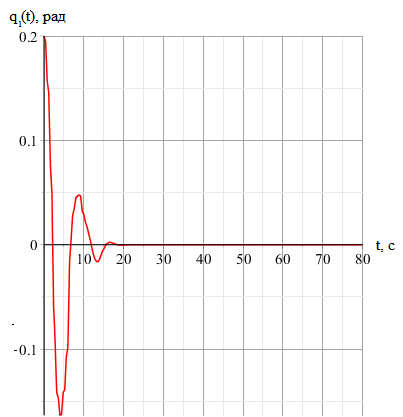
\includegraphics{3chain_1}
    	\caption{Зависимость угла поворота первого звена от времени при управлении (3.6) }
    	\label{fig:manip31}
    \end{figure}
    
    \begin{figure}[h]
    	\centering
    	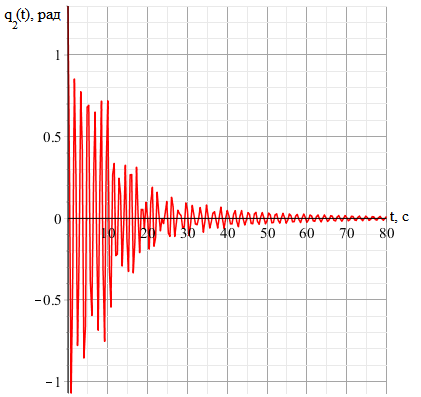
\includegraphics{3chain_2}
    	\caption{Зависимость угла поворота второго звена от времени при управлении (3.6)  }
    	\label{fig:manip32}
    \end{figure}
    
    \begin{figure}[h]
    	\centering
    	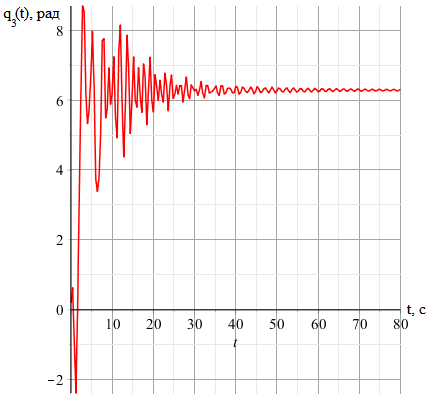
\includegraphics{3chain_3}
    	\caption{Зависимость угла поворота третьего звена от времени при управлении (3.6) }
    	\label{fig:manip33}
    \end{figure}
   
 
  \section{Синтез управления в задаче о стабилизации нестационарного программного движения манипулятора}% 
 Рассмотрим решение задачи стабилизации в области $G = {(x, \dot x) \in R^6 : \|x\| < \varepsilon, \quad \|\dot x \| < \varepsilon, \quad \varepsilon = const>0}$
 с помощью непрерывного управления вида
 
 \begin{equation}
  Q^{(1)} (x, \dot x) = B(\dot x + p(x)),
  p^{'}(x) = (\sin \frac{x_1}{2}, \sin \frac{x_2}{2}, \sin \frac{x_3}{2})
 \end{equation}
 
 где $B \in R^{3 \times 3}$ есть матрица коэффициентов усиления сигналов, подлежащая определению; $p(x)$ --- непрерывно дифференцируемая вектор-функция, такая, что $\| p(x) \| \ge p_0(x) > 0, p_0(0) = 0$.
 Возьмем для системы (3.3) вектор-функцию Ляпунова $V = (V^1, V^2)^{'}$ с коэффициентами вида $V^1 = \|p(x)\|, \quad V^2 = \sqrt{(\dot x + p(x))^{'} A^{(1)} (t, x) (\dot x + p(x))}$.
 
 Вычисляя производные по времени от квадратов компонент вектор-функции Ляпунова  в силу системы (3.3), получим 
 
 \begin{equation*}
 \begin{array}{c}
 \displaystyle \frac{d}{dt} (V^1(x))^2 = 2 V^1 \dot V^1 = 2 p^{'} \dot p = 2 p^{'} \frac{\partial p }{\partial x} \dot x = -2 p^{'} \frac{\partial p }{\partial x} p + 2 p^{'} \frac{\partial p }{\partial x}(\dot x + p),\\
    \displaystyle \frac{d}{dt} (V^2(x))^2 = 2 V^2 \dot V^2 =\\
   \displaystyle = 2(\ddot x + \dot p)^{'} A^{(1)} (\dot x + p) + (\dot x + p)^{'} \dot A^{(1)} (\dot x + p) =\\
   \displaystyle = 2(- C^{(1)}(t, x, \dot x) \dot x - K(t, x) + Q^{(1)}(x, \dot x) + Q^{(2)}(t, x, \dot x))^{'} (\dot x + p) +\\
   \displaystyle + 2 \dot p^{'} A^{(1)} (\dot x + p) + (\dot x + p)^{'} \dot A^{(1)} (\dot x + p).
 \end{array}
 \end{equation*}
 
 Отсюда получим следующие оценки:
 $$\dot V^1 \le - \mu_1 V^1 + \frac{m_1}{\lambda(t, x)} V^2, \quad \dot V^2 \le \frac{m_2}{\lambda(t, x)} V^1 - \frac{\mu_2}{\lambda^2(t,x)},$$
 
 где положительные постоянные $\mu_2, \mu_2, m_1, m_2$  и функция $\lambda(t,x)$  определяются из следующих условий:
 \begin{equation}
 p^{'} \frac{\partial p}{\partial x} p \ge \mu_1 \|p\|^2, \quad \left| \left| \frac{\partial p}{\partial x} \right| \right| \le m_1, \lambda(t, x) \| \dot x + p \| = V^2,
 \end{equation}
 
 \begin{equation}
 \| Q^{(2)} (t, x, \dot x) \le \left( m_2 - \left| \left| C^{(1)}(t, x, \dot x) + K - A^{(1)}(t, x) \frac{\partial p}{\partial x}\right| \right| \right) \|p\|
 \end{equation}

\begin{equation}
 \lambda_{max} \left( B + B^{'} - K - K^{'} + A^{(1)}(t, x) \frac{\partial p}{\partial x} + \left( \frac{\partial p}{\partial x} \right) ^{'} A^{(1)}(t, x) \right) \le -2 \mu_2
\end{equation}
 
 Здесь $\lambda_{max}(\cdot)$ есть максимальное собственное значение соответствующей матрицы. 
 Тогда для системы (3.3) можно построить следующую систему сравнения:
 
 \begin{equation}
 \dot u^1 = - \mu_1 u^1 + \frac{m_1}{\lambda(t,x)} u^2, \dot u^2 = \frac{m_2}{\lambda(t, x)} u^1 - \frac{\mu_2}{\lambda^2(t, x)} u^2. 
 \end{equation}
 
 Согласно теореме сравнения об экспоненциальной устойчивости \cite{peregudova14} из свойства экспоненциальной устойчивости нулевого решения системы сравнения (3.5) следует аналогичное свойство нулевого решения системы (3.3).  Можно показать, что нулевое решение системы сравнения (3.5) будет экспоненциально устойчиво при следующем условии
 $$4 \mu_1 \mu_2 > (m_1 / k + m_2 k)^2, \quad k = const>0.$$
 
 Численное моделирование движения манипулятора при действии управления (3.4) проводилось при следующих значениях параметров манипулятора и программной траектории
 
\begin{equation*}
\begin{array}{l}
 m_2=15 \text{ кг}, \quad m_3=2,5 \text{ кг}, \quad m_0 = 2 \text{ кг}, \quad l_2 = 1 \text{ м}, \quad r_2=0,5 \text{ м}, \quad r_3 = 0,5 \text{ м},\\
 \quad J_{01} = 0,1 \text{ кг} \cdot \text{м\textsuperscript{2}}, \quad q_1^0(t) = 0,2t, \quad q_2^0(t) = 1,5 + 0,5 \sin{t}, \quad q_3^0(t) = 0,5 \sin{(0,5 t)}.
\end{array}
\end{equation*}
 
 На рисунках 3.5–3.7 представлены результаты моделирования. Пунктирной линией обозначены  составляющие программного движения, а сплошной – реального движения системы.
 
 
  \begin{figure}[h]
  	\centering
  	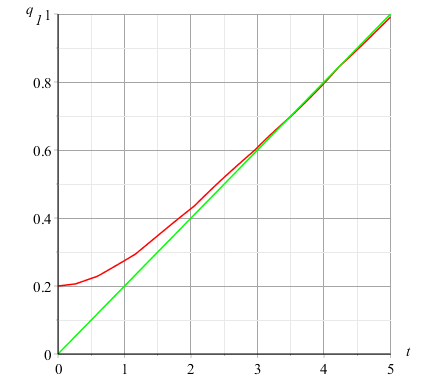
\includegraphics{pic1}
  	\caption{Зависимость угла поворота первого звена от времени при управлении (3.4) }
  	\label{fig:manip2}
  \end{figure}
  
  \begin{figure}[h]
    	\centering
    	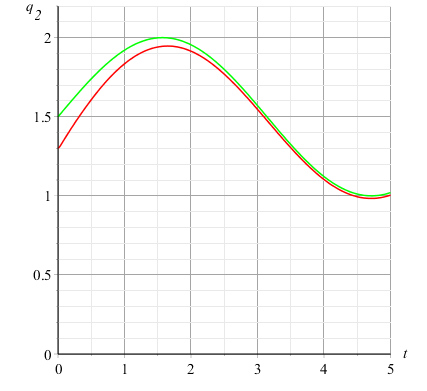
\includegraphics{pic2}
    	\caption{Зависимость угла поворота второго звена от времени при управлении (3.4)  }
    	\label{fig:manip2}
    \end{figure}
    
      \begin{figure}[h]
      	\centering
      	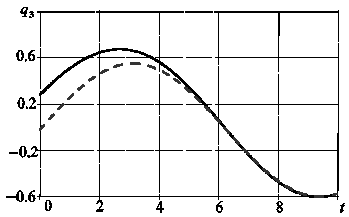
\includegraphics{pic3}
      	\caption{Зависимость угла поворота третьего звена от времени при управлении (3.4) }
      	\label{fig:manip2}
      \end{figure}